\section{Galaxy}

\begin{frame}{Refs}
The Gaia-ESO Survey: the Galactic Thick to Thin Disc transition
''The Formation and Evolution of the Milky Way: The distribution of the chemicalelements in our galaxy serves as a "fossil record" of its evolutionary history''
''Stellar Populations and the Formation of theMilky Way'' (Majewski)
\end{frame}

\subsection{Primordial composition and nucleosynthesis}

\subsection{Via Lattea e gruppo locale. Teorie di formazione galattica}

\begin{frame}{Milky way: thin/thick disk, halo}
\begin{columns}[T]
\begin{column}{0.6\textwidth}
\begin{figure}[!ht]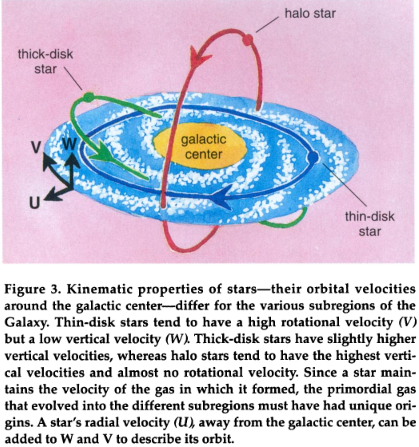
\includegraphics[trim={0cm 0cm 0 0},clip, keepaspectratio,width=0.99\textwidth]{MWcartoon}\label{fig:MWcartoon}\end{figure}
\end{column}
\begin{column}{0.4\textwidth}
Thin: $\exv{z}\approx\SI{300}{\parsec}$, Pop I (many metals absorption lines $Z\approx0.013$)
Thick: $\exv{z}\approx\SI{1000}{\parsec}$, Pop II (absorption line almost. from H: $Z<0.004$)-Int pop I; kinemat. hot, old, $\alpha$-enh metal poor.
Halo: Extreme pop II ($[\alpha/Fe]\approx0.3$)
\end{column}
\end{columns}
\end{frame}

\begin{frame}{Milky way: chemical evolution}
\begin{columns}[T]
\begin{column}{0.6\textwidth}
\begin{figure}[!ht]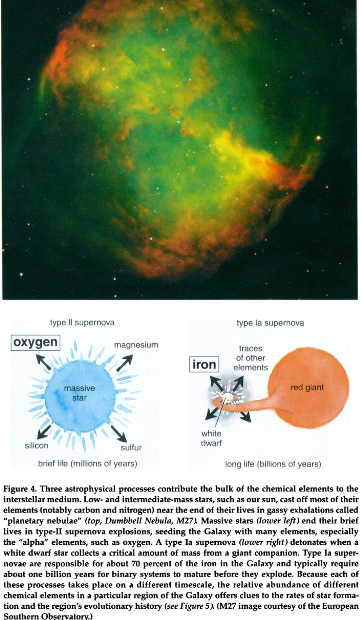
\includegraphics[trim={0cm 0cm 0 0},clip, keepaspectratio,height=0.89\textheight]{PNSNISNII}\label{fig:PNSNISNII}
\end{figure}
\end{column}
\begin{column}{0.4\textwidth}
Massive star: oxigen/$\alpha$-elements (Ne, Mg, S, Si)
\end{column}
\end{columns}
\end{frame}


\subsection{Popolazioni stellari}

\subsection{cluster stellari}

\begin{frame}{Distanza ammassi}
main sequence fitting
tip rgb
ZAHB
clump elio
RR lyrae
cefeidi
\end{frame}

\begin{frame}{indicatori di et\'a}
Turn-off/overall contraction: Isocrone di ammassi giovani/vecchi; metodo orizzontale e vertical per ammassi antichi; Lithium depletion boundary per datazione di ammassi giovani
\end{frame}

\begin{frame}{Indicatori di He (e Z??)}
??
\end{frame}

\section{Star formation - IMF}

\begin{frame}{Popolazioni in galassie esterne}
star formation history; popo non risolte semplici e complesse
\end{frame}